\documentclass[10pt]{article}

% page setup
\usepackage{geometry}
\geometry{a4paper, left=4.8cm, right=4.8cm, top=4.4cm, bottom=4.4cm}
% \usepackage{ragged2e}
% \setlength{\RaggedRightParindent}{\parindent}

% language settings
\usepackage[british]{babel}
\usepackage{csquotes}

% maths
\usepackage{amsmath, amssymb}
\usepackage{mathtools}
\usepackage{bm}
\newcommand{\I}{\mathbb{I}}
\newcommand{\B}{\symbf{\beta}}
\newcommand{\bz}{\bar{\symbf{z}}}
\newcommand{\ssm}{\smallsetminus}
\newcommand{\w}{\symbf{w}}
\newcommand{\Tau}{\symbf{\tau}}
% \renewcommand{\Pr}{\text{Pr}}
% \renewcommand{\max}{\text{max}}
\usepackage{siunitx}

% typography
\usepackage[dvipsnames]{xcolor}
\usepackage[hidelinks, colorlinks=true, allcolors=Emerald, bookmarks=false]{hyperref}
\usepackage{microtype}
\usepackage{booktabs}

% Libertinus
\usepackage{fontspec}
% \setsansfont[Numbers=OldStyle]{Gill Sans}
\setsansfont[Numbers=OldStyle]{TeX Gyre Adventor}
% \usepackage[osf]{carlito}
% \usepackage[medium]{inter}
\usepackage[otfmath]{XCharter}

% \usepackage{fontspec}
% \defaultfontfeatures{Ligatures=TeX, Numbers=OldStyle}
% \setmainfont{Georgia}
% \setsansfont[Numbers=OldStyle]{Gill Sans}
% % \newfontfamily\cabin{Cabin Regular}[Numbers=OldStyle]
% % \usepackage[charter,expert]{mathdesign}
% \usepackage{unicode-math}
% \setmathfont[Numbers=Lining]{XCharter-Math.otf}

% sections
\usepackage{sectsty}
\allsectionsfont{\fontsize{13pt}{17pt}\selectfont\normalfont\sffamily}

% \makeatletter
% \def\@seccntformat#1{\cabin\csname the#1\endcsname\quad}
% \makeatother

% line spacing
\usepackage{setspace}
\setstretch{1.3}
\usepackage[all]{nowidow}

% bibliography
\usepackage[round]{natbib}
\bibliographystyle{chicago}

% figures
\usepackage{tikz}
\usetikzlibrary{bayesnet}
\usetikzlibrary{arrows}
\usepackage{graphicx}
\usepackage[labelfont=it, format=hang]{caption}
\usepackage{float}


\begin{document}

% \RaggedRight\

{\noindent\fontsize{15pt}{18pt}\selectfont \textsf{TreeWAS:\@ Model and Algorithms}}\\[20pt]
 Lino A.\hspace{0.08333em}F.\ Ferreira\\11 July 2020\\[20pt]


\noindent These notes describe the TreeWAS model and associated inference algorithms introduced by~\cite{Cortes2017}.

\section{Model description}\label{subsec:modeldesc}

Consider a sample of $N$ individuals indexed by $i$. For each individual $i$, we observe a series of binary indicators $z_{ij}$, with $j=1,\ldots,J$, taking the value 1 if this individual has a particular phenotype and 0 otherwise.
The indicators $z_{ij}$ are indexed according to a hierarchical tree structure, %(this structure is the same for all individuals)
with each indicator corresponding to a node in the tree (1, or equivalently $A$, is the index of the root node). In our context, the phenotypic indicators represent an ontology of diseases, with increasingly specific disease categories as we move down the tree.
We will model these disease indicators $z_{ij}$ as being the realised values of binary random variables $Z_{ij}$ and denote this output process by $\{\symbf{Z}_i\}_{i=1}^N$, with $\symbf{Z}_{i} = (Z_{iA},\ldots,Z_{iJ})$.

We also consider a number of different genetic loci indexed by $s$, with $s=1,\ldots,S$. At a particular locus $s$, the categorical indicator $G_{is}$ takes the value 0 if individual $i$ is homozygous for the reference allele at that locus, the value 1 if they are heterozygous and the value 2 if they are homozygous for the alternative allele.

For a \textit{terminal (or leaf) node} $l$ in the tree, the probability that the random variable $Z_{il}$ takes value 1 given data $G_{is}$ is assumed to follow a logistic model:
\begin{align}
  \Pr(Z_{il}=1|Y_{ils}) = \frac{e^{Y_{ils}}}{1 + e^{Y_{ils}}}, \label{eq:emission}
\end{align}
where $\Pr(\cdot)$ is the probability mass function (p.m.f.).\footnote{In a slight abuse of notation, $\Pr(\cdot)$ may denote either a p.m.f. or a probability density function (p.d.f.) depending on the context.} 
$Y_{ils}$ is defined for a subject $i$, a terminal node $l$ and a variant $s$ as follows:
\begin{align*}
  Y_{ils} = \beta_{ls}^0 + \beta_{ls}^1 \I(G_{is}=1) + \beta_{ls}^2\I(G_{is}=2),
\end{align*}
where $\I(\cdot)$ is the indicator function, $\beta_{ls}^0$ is the intercept term and $\beta_{ls}^1$ and $\beta_{ls}^2$ are separate coefficients for the heterozygous and homozygous states, respectively. From now on, we will consider a single generic locus $s$ and drop the subscript to simplify notation.

We associate with each node $j$ in the tree a length-3 vector of coefficients $(\beta^0_j,\beta^1_j,\beta^2_j)$ and model the pairs $(\beta_j^1, \beta_j^2)$ as evolving down a tree with the same structure as that of the output process. Given parameter vector $(\theta,\pi_1)$ the coefficients of a parent node are inherited with probability $e^{-\theta}$ and transition to a new pair of values with probability $1-e^{-\theta}$. In the latter case, the new values are $(0,0)$ with probability $1-\pi_1$ while with probability $\pi_1$ they are drawn from a joint prior $f(\beta_j^1,\beta_j^2)$. Writing $\B_j=(\beta_j^1,\beta_j^2)$, $f(\B_j)$ is assumed to be the following:
\begin{align}
  f(\B_j) \propto \mathcal{N}_2(\symbf{0},\Sigma) \cdot {\left\lVert (\beta_j^1, \beta_j^2/2) \right\rVert}^k \cdot \epsilon, \label{eq:prior}
\end{align}
where $\mathcal{N}_2$ is a bivariate Normal density with mean vector $\symbf{0}=(0,0)$ and covariance matrix $\Sigma$,
\begin{align*}
  \Sigma =
  \begin{bmatrix}
    \sigma_1^2 & r\sigma_1\sigma_2\\
    r\sigma_1\sigma_2 & \sigma_2^2
  \end{bmatrix}
\end{align*}
for some $\sigma_1\geq0$, $\sigma_2\geq0$ and $r\in\mathbb{R}$, and
\begin{align*}
  \epsilon = \left\{\begin{array}{ll}
        0.1, & \quad\text{if } \beta_j^1\beta_j^2 < 0\\
        0.1, & \quad\text{if } |\beta_j^1| > |\beta_j^2|\\
        1,   & \quad\text{otherwise.}
        \end{array}\right.
\end{align*}
Note that the p.d.f.\ in equation (\ref{eq:prior}) is only specified up to a constant of proportionality. The mixture distribution for $\B_j$ in the case where a child node does not inherit its parents' coefficients is denoted by $f^*(\beta_j^1,\beta_j^2)$. This is also the distribution from which $\B_A$, the vector of coefficients of the root node, is drawn. \cite{Cortes2017} use the following parameter values: $\pi_1=0.001, \theta=1/3, \sigma_1 = 2, \sigma_2 = 4, k=0.5$ and $r=0.5$.

We make no explicit assumption on the evolution of the $\beta_j^0$ coefficients. When fitting the model as we describe in the next section, the intercept term will be chosen, for each node $j$, to maximise the likelihood of the observed data at that node, $\symbf{z}_j=(z_{1j},\ldots,z_{Nj})$. Figure~\ref{fig:treewas} shows an example of the TreeWAS graphical model.

 \begin{figure}[h!]
   \centering
   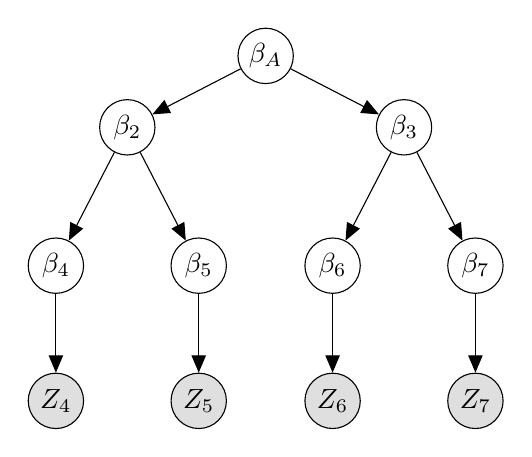
\begin{tikzpicture}
     % root
     \node[latent] (anc) {$\B_A$};%
     % second row
     \node[latent, below left=0.4cm and 1.25cm of anc] (2) {$\B_2$};%
     \node[latent, below right=0.4cm and 1.25cm of anc] (3) {$\B_3$};%
     % third row 
     \node[latent, below left=1.25cm and 0.4cm of 2] (4) {$\B_4$};%
     \node[latent, below right=1.25cm and 0.4cm of 2] (5) {$\B_5$};%
     \node[latent, below left=1.25cm and 0.4cm of 3] (6) {$\B_6$};%
     \node[latent, below right=1.25cm and 0.4cm of 3] (7) {$\B_7$};%
     % output
     \node[obs, below=1cm of 4] (z4) {$Z_4$};%
     \node[obs, below=1cm of 5] (z5) {$Z_5$};%
     \node[obs, below=1cm of 6] (z6) {$Z_6$};%
     \node[obs, below=1cm of 7] (z7) {$Z_7$};%
     % edges
     \edge {anc} {2};
     \edge {anc} {3};
     \edge {2} {4};
     \edge {2} {5};
     \edge {3} {6};
     \edge {3} {7};
     \edge {4} {z4};
     \edge {5} {z5};
     \edge {6} {z6};
     \edge {7} {z7};
   \end{tikzpicture}
   \caption{Example tree of disease coefficient pairs $\B$ and terminal disease indicator nodes $Z$. Only the realised values of the disease indicators (shaded in grey) are observed.}\label{fig:treewas}
 \end{figure}

Crucially, note that internal nodes are \textit{not} drawn from a logistic model like the one specified in equation (\ref{eq:emission}). In fact, internal disease nodes are not included in the probabilistic graphical model (see Figure \ref{fig:treewas}) and so we do not write their distribution. While it would be natural to model every node in the tree through a logistic model as above (this would give us a Hidden Markov Tree Model (HMTM)~\citep{Crouse1998}) this would not be compatible with the ontological nature of the disease tree.

To see this, note that the value of every internal node in the disease tree is uniquely determined by that of its children.\footnote{For example, consider a parent node corresponding to respiratory infection whose children are nodes corresponding to pneumonia, lung abscess and empyema. If an individual has pneumonia, lung abscess or empyema, then they necessarily have a respiratory infection, and therefore the parent node will take value 1. On the other hand, if they do not have any of these three kinds of respiratory infection then the parent node will take value 0.} By this argument, we can say that, conditional on the observed values for its children $\gamma(j)$, the value of an internal node $j$ is fixed (we can write $z_{ij} = \max \left\{z_{ik} : k\in\gamma(j)\right\}$ for all $i$) which is not compatible with each node being stochastically determined based only on its $\B$ coefficient vector.

% If a parent node takes value 0 then so must its children.\footnote{For example, if an individual does not have a cardiovascular condition then they do not have hypertension since this is a sub-type of cardiovascular disease.}
% Similarly, if we observe all the children of a parent node then we know the value of this node.
The TreeWAS model is thus a simplified version of the HMTM model where only the terminal hidden state nodes have an associated output with emission distribution specified by equation~(\ref{eq:emission}) and only data for the annotations associated with these terminal nodes is used to estimate the model.


\section{Model fitting}

In fitting the model to data, our first goal is to assess, for each genetic locus, whether there is evidence of association between variation at that locus and at least one of the
phenotypes in the tree. Having established this, we can then concentrate on those loci for which such evidence of association exists and examine the posterior distributions of the different $\B_j$ in their trees. %This will allow us to identify variants with an effect on specific disease phenotypes while taking into account the correlation structure between effects for similar diseases.

The first task is one of model comparison between a model under which no evidence of association exists (i.e.\ $\symbf{\beta_j}=(0,0)$ for all nodes $j$ in the tree) and an alternative model under which there is evidence of association with \textit{at least one} phenotype. The latter model encompasses all instances where at least one coefficient differs from 0.

In keeping with our Bayesian framework, we will use a Bayes Factor to compare these two models. This requires us to compute the integrated likelihood (also known as marginal likelihood or model evidence) of our data under the two scenarios. Defining, for simplicity of notation, a vector $\B \coloneqq (\B_A,\ldots,\B_J)$ and denoting the terminal output data $\left\{\symbf{z}_l\right\}_{l=1}^N$ by $\symbf{z}$,\footnote{Note that only the most specific disease categories are included in $\symbf{z}$: none of the internal nodes $z_j$ are included in this model.} we write the integrated likelihood for the model of no association, denoted $L_\varnothing$, as follows:
\begin{align*}
  L_\varnothing = \int \Pr( \symbf{z}, \B |
  \B = \symbf{0})\, d\B,
\end{align*}
where $\Pr(\cdot)$ is now a p.d.f.\ and $\symbf{0}$ is a zero vector of length $2J$. Since there is only one way in which all coefficients can be zero, this can be simplified:
\begin{align*}
  L_\varnothing = \Pr( \symbf{z} | \B = \symbf{0}).
\end{align*}

In contrast with the model of no association, there are many (in fact, an infinite number of) ways in which at least one of the model coefficients can differ from zero. Because of this, directly computing the integrated likelihood under the alternative model (denoted $L_+$) would be intractable. To avoid this issue, we note that the full integrated likelihood $L_\text{full}$, which is defined as
\begin{align}
  L_\text{full} = \int \Pr( \symbf{z}, \B)\, d\B, \label{eq:lfull1}
\end{align}
can be written as the weighted sum of the null model and alternative model likelihoods:
\begin{align}
  L_\text{full} = \pi_\varnothing L_\varnothing + (1-\pi_\varnothing) L_+, \label{eq:lfull2}
\end{align}
where $\pi_\varnothing$ is the prior probability of all coefficients being zero. For a tree with $J$ nodes, this prior probability is equal to:
\begin{align*}
  \pi_\varnothing = (1-\pi_1) \cdot
  {\left[e^{-\theta} + (1-e^{-\theta})(1-\pi_1)\right]}^{J-1}.
\end{align*}
Equation (\ref{eq:lfull2}) implies that, if we can compute the full and null model likelihoods, we can easily obtain $L_+$. We can then compute the Bayes Factor to test the null hypothesis of no association against the alternative hypothesis of at least one association:
\begin{align*}
  \text{BF}_\text{tree} = \frac{L_+}{L_\varnothing}.
\end{align*}

Computing the full integrated likelihood $L_\text{full}$ requires numerically evaluating a high-dimensional integral, an expensive operation. \cite{Cortes2017} do this via a recursive algorithm iterating upwards from the terminal nodes of the tree, which makes the computation much more tractable. A small modification of this algorithm then allows for computing $L_\varnothing$.

A short description of the upward recursive algorithm is as follows: we start by evaluating the likelihood of observing the phenotypic data $\bz_l$ for each terminal node $l$ on the tree for a grid of $\B$ values. Moving up one level, we note that the likelihood of an internal node is equal to the likelihood of observing all of its children, which are independent of one another.\footnote{This is because the value of a parent node is uniquely determined by those of its children.} We thus compute the parents' likelihoods for a grid of $\B$ values by multiplying those of their children, and in doing so must integrate over all the values of the children's $\B$ coefficients (these are weighted by the prior $f^*(\B_l)$). 
We proceed in this manner until reaching the root node. A detailed derivation of this algorithm is given in Appendix~\ref{sec:upward}.

We then turn to the question of how to obtain the posterior distributions of the $\B_j$ coefficients for those variants for which some evidence of association is found. This requires a second algorithm which proceeds downwards from the root node towards the terminal nodes of the tree, described in detail in Appendix~\ref{sec:downward}.

Together, these two algorithms are very similar to the the Upward-Downward Algorithm~\citep{Crouse1998} for HMTMs, which in turn is reminiscent of the Forward-Backward Algorithm used for Hidden Markov Models. The presentation of the TreeWAS algorithms in Appendices~\ref{sec:upward} and~\ref{sec:downward} follows closely that in~\cite{Durand2004}, although we aim to keep the notation as consistent as possible with that of~\cite{Cortes2017} and account for the different structure of our graphical model. 


\bibliography{ref.bib}




\clearpage
\appendix
\section{Upward recursive algorithm}\label{sec:upward}

We begin by establishing some additional notation: following~\cite{Durand2004}, we define $\bar{Z}_{ij}$ as the \textit{terminal nodes of the subtree} of disease indicators rooted at node $j$ for individual $i$, so that $\bar{Z}_{iA}$ is the set of all leaf nodes for that individual. $\bar{\symbf{Z}}_{j}$ is then the set of terminal nodes of the subtrees rooted at $j$ for all individuals, and as before $\bz_{j}$ is their realised value, i.e.\ the observed data.


We aim to compute the full integrated likelihood $L_\text{full}$:
\begin{align*}
  L_\text{full} &= \int \Pr( \bz_A, \B )\, d\B
                  = \Pr( \bz_A).
\end{align*}
Applying simple rules of probability, this can also be written as
\begin{align}
  L_\text{full} &= \Pr( \bz_A) \nonumber\\
                &= \int \Pr( \bz_A, \B_A )\, d\B_A \nonumber\\
  &= \int \Pr( \bz_A | \B_A ) f^*(\B_A)  \, d\B_A. \label{eq:lfull3}
\end{align}


Following~\cite{Cortes2017}, we now make two further definitions which will simplify the notation below. We first define $F_j(\B_j)$ as the probability of observing the subtree $\bz_j$ given only the coefficients $\B_j$ for node $j$, that is:
\begin{align*}
  F_j(\B_j) \coloneqq \Pr(\bz_j | \B_j).
\end{align*}
Secondly, and defining $\rho(j)$ as the parent node of $j$, we define $G_j(\B_{\rho(j)})$ as the probability of observing the subtree $\bz_j$ given only the coefficients $\B_{\rho(j)}$ for \textit{the parent of node} $j$, that is:
\begin{align*}
  G_j(\B_{\rho(j)}) \coloneqq \Pr(\bz_j | \B_{\rho(j)}).
\end{align*}
This now allows us to simplify equation (\ref{eq:lfull3}) as follows:
\begin{align*}
  L_\text{full} &= \int F_A(\B_A) f^*(\B_A)  \, d\B_A.
\end{align*}


The key point is that, instead of doing high-dimensional integration to obtain $\Pr(\bz_A)$ as in equation (\ref{eq:lfull1}), we can perform this integration recursively starting from the terminal nodes of the tree. To see this, we start by noting that, for a terminal node $l$, $\bz_l=\symbf{z}_l$. Then, $F_l(\B_l)$ is simply equal to $\Pr(\symbf{z}_l|\B_l)$. Moreover, assuming independent observations we have $\Pr(\symbf{z}_l | \B_l) = \prod_{i=1}^N \Pr(z_{il} | \B_l)$.


For an internal node $j$, and defining $\gamma(j)$ as the children of $j$, we can rewrite $F_j(\B_j)$ as follows:
\begin{align*}
  F_j(\B_j) &\coloneqq \Pr(\bz_j | \B_j) \nonumber\\
            &= \prod_{k\in\gamma(j)} \Pr(\bz_k | \B_j )\\
            &= \prod_{k\in\gamma(j)} G_k(\B_j).
\end{align*}


We now note that $G_k(\B_j)$ can also be rewritten:
\begin{align}
  G_k(\B_j) &\coloneqq \Pr(\bz_k | \B_j) \nonumber\\
            &= \int \Pr(\bz_k,\B_k | \B_j) \,d\B_k \nonumber\\
  &= \int \underbrace{\Pr(\bz_k | \B_k)}_{=F_k(\B_k)} \Pr(\B_k | \B_j)   \,d\B_k, \label{eq:g}
\end{align}
where the last equality follows from the HMTM setup, which implies that the terminal phenotypes $Z_{ik}$ are independent (for all $i$) of the coefficients of their associated parent coefficients, in this case $\B_j$, when conditioned on their own associated coefficients $\B_k$.


The model setup described in Section~\ref{subsec:modeldesc} also implies the following expression for $\Pr(\B_k | \B_j)$:
\begin{align*}
  \Pr(\B_k | \B_j) = e^{-\theta} \delta(\B_k - \B_j) + (1-e^{-\theta})f^*(\B_k),
\end{align*}
where $\delta(\cdot)$ is the Dirac delta function. Equation (\ref{eq:g}) then becomes:
\begin{align}
  G_k(\B_j) &= \int F_k(\B_k) \left[ e^{-\theta} \delta(\B_k - \B_j) + (1-e^{-\theta})f^*(\B_k) \right]  \,d\B_k \nonumber\\
            &= e^{-\theta} \int F_k(\B_k) \delta(\B_k - \B_j) \,d\B_k +
              (1-e^{-\theta}) \int F_k(\B_k) f^*(\B_k) \,d\B_k. \label{eq:g2}
\end{align}
Noting that
\begin{align*}
  \int F_k(\B_k) \delta(\B_k - \B_j) \,d\B_k = F_k(\B_j)= \Pr(\bz_k | \B_j),\footnotemark
\end{align*}
\footnotetext{This is known as the \textit{sifting property} of the delta function.}and defining a new function $L_k$ as
\begin{align*}
 L_k \coloneqq \int F_k(\B_k) f^*(\B_k) \,d\B_k,
\end{align*}
equation (\ref{eq:g2}) becomes
\begin{align*}
  G_k(\B_j) &= e^{-\theta} F_k(\B_j) +
              (1-e^{-\theta}) L_k.
\end{align*}


To summarise, these are the key equations of the upward recursive algorithm used to compute the full integrated likelihood $L_\text{full}$:
\begin{align}
  L_\text{full} &= \int F_A(\B_A) f^*(\B_A)  \, d\B_A \label{eq:sum_lfull}\\
  F_l(\B_l) &= \Pr(\symbf{z}_l|\B_l), && \text{for a terminal node $l$} \label{eq:sum_f1}\\  
  F_j(\B_j) &= \prod_{k\in\gamma(j)} G_k(\B_j), && \text{for an internal node $j$} \label{eq:sum_f2}\\
  G_k(\B_j) &= e^{-\theta} F_k(\B_j) + (1-e^{-\theta}) L_k \label{eq:sum_g}\\
  L_k &= \int F_k(\B_k) f^*(\B_k) \,d\B_k. \label{eq:sum_lk}
\end{align}


The algorithm is then as follows:
\begin{enumerate}
\item Initialise by computing $F_l(\B_l)$ for all the terminal nodes in the tree using equation (\ref{eq:sum_f1}). This involves computing $\Pr(\symbf{z}_l|\B_l)$ for each terminal node $l$ for a grid of values for $\B_l=(\beta_l^1,\beta_l^2)$.

  As mentioned above, $\beta_l^0$ is chosen, for each value of $\B_l=(\beta_l^1,\beta_l^2)$, to maximise the likelihood for our logistic model. Since maximum likelihood estimation of the logistic regression model does not have a closed form solution, this must be done numerically for each pair $\B_l=(\beta_l^1,\beta_l^2)$ in the grid.

 For each terminal node $l$, also compute $L_l$ using equation (\ref{eq:sum_lk}) and $G_l(\B_{\rho(l)})$ for a grid of values for $\B_{\rho(l)}$ using equation (\ref{eq:sum_g});
  
\item Move up one level and compute $F_{\rho(l)}(\B_{\rho(l)})$ using equation (\ref{eq:sum_f2}).

  Also compute $L_{\rho(l)}$ and $G_{\rho(l)}$ for a grid of values as before;
  
\item Continue recursively in this way until reaching the root node and obtaining $F_A(\B_A)$;
  
\item Finally, evaluate equation (\ref{eq:sum_lfull}) to obtain $L_A=L_\text{full}$.
\end{enumerate}
Note that, using this algorithm, we integrate only over two variables (the different $\B_j$ pairs) at a time. In choosing the $\beta^0$ coefficients to maximise the likelihood, we avoid having to also integrate over them.


Finally, we compute the likelihood of all leaf disease nodes taking value 0, i.e.\ $L_\varnothing = \Pr(\bz | \B = \symbf{0})$, as follows:
\begin{align*}
  L_\varnothing = \prod_{l\in T} \Pr(\symbf{z}_l|\B_l = \symbf{0}).
\end{align*}

% Add bit about how using beta rather than some realised beta' is a bit of an abuse of notation.




\section{Downward recursive algorithm}\label{sec:downward}

The upward recursion algorithm described in the previous section allows us to compute the full and null likelihoods and, consequently, the likelihood for the model of at least one association. As described above, this can then be used to obtain a Bayes Factor for assessing, for each genetic locus, the evidence of association between this locus and any of the terminal node phenotypes in the tree. Having identified those loci for which such evidence exists, we proceed to deriving the posterior distributions of the different $\B_j$ coefficients for these loci. This in turn allows us to quantify the evidence of association between a variant and specific disease phenotypes.


We now describe the downward recursion algorithm used to obtain the posterior distributions of the model's coefficients. First, for a node $j$, the posterior distribution of $\B_j$ given the data for all terminal nodes $\bz_A$ can be written as follows:
\begin{align}
  \Pr(\B_j | \bz_A) = \frac{\Pr(\B_j, \bz_A)}{\Pr(\bz_A)}. \label{eq:post}
\end{align}
Since we now know how to obtain $\Pr(\bz_A)=L_A$, by computing the joint distribution $\Pr(\B_j, \bz_A)$ we can obtain the posterior of $\B_j$.


Again following~\cite{Durand2004}, if $Z_{ik}$ is a proper subtree of $Z_{ij}$, we define $\bar{Z}_{ij\ssm k}$ as the \textit{leaf} indicators of the subtree rooted at node $j$ for individual $i$ \textit{except for the leaf nodes of the subtree rooted at $k$ for the same individual}. Then, $\bz_{A\ssm j}$ is all the observed data except for that of subtree $\bz_j$.


We can then rewrite $\Pr(\B_j, \bz_A)$ as follows:
\begin{align}
  \Pr(\B_j, \bz_A) &= \Pr(\B_j, \bz_j, \bz_{A\ssm j})\nonumber\\
  &= \Pr(\bz_j | \B_j, \bz_{A\ssm j}) \Pr(\B_j, \bz_{A\ssm j})\nonumber\\
  &= \underbrace{\Pr(\bz_j | \B_j)}_{=F_j(\B_j)} \, \Pr(\B_j, \bz_{A\ssm j}), \label{eq:pbz}
\end{align}
where the last equality follows from the fact that $\bar{\symbf{Z}}_j$ is independent of $\bar{\symbf{Z}}_{A\ssm j}$ when conditioned on $\B_j$. By defining a further function
\begin{align*}
  B_j(\B_j) \coloneqq \Pr(\B_j, \bz_{A\ssm j}),
\end{align*}
we can write $\Pr(\B_j, \bz_A)$ simply as
\begin{align}
  \Pr(\B_j, \bz_A) = F_j(\B_j) B_j(\B_j). \label{eq:B1}
\end{align}


We now show how $B_j(\B_j)$ can be computed through a downward recursion from the root towards the terminal nodes of the tree. For any node other than the root node $A$, we have:
\begin{align*}
  B_j(\B_j) &\coloneqq \Pr(\B_j, \bz_{A\ssm j})\\
            &= \int \Pr(\B_j, \B_{\rho(j)}, \bz_{A\ssm \rho(j)}, \bz_{\rho(j)\ssm j}) \,d\B_{\rho(j)}\\
            &= \int \underbrace{\Pr(\B_j | \B_{\rho(j)})}_{=q(\B_j,\B_{\rho(j)})}
              \, \Pr(\B_{\rho(j)}, \bz_{A\ssm \rho(j)}, \bz_{\rho(j)\ssm j}) \,d\B_{\rho(j)},
\end{align*}
where we denote the transmission distribution of $\B_j$ given its parent $\B_{\rho(j)}$ by $q(\B_j,\B_{\rho(j)}) \coloneqq \Pr(\B_j | \B_{\rho(j)})$.
Applying the definition of conditional probability and noting that $\bar{\symbf{Z}}_{\rho(j)}$ is independent of $\bar{\symbf{Z}}_{A\ssm \rho(j)}$ when conditioned on  $\B_{\rho(j)}$, we have:
\begin{align}
  B_j(\B_j)  &= \int q(\B_j,\B_{\rho(j)}) \Pr(\bz_{\rho(j)\ssm j} | \B_{\rho(j)}, \bz_{A\ssm \rho(j)}) \,
              \underbrace{\Pr(\B_{\rho(j)}, \bz_{A\ssm \rho(j)})}_{=B_{\rho(j)}(\B_{\rho(j)})} \,d\B_{\rho(j)} \nonumber\\
            &= \int q(\B_j,\B_{\rho(j)}) \Pr(\bz_{\rho(j)\ssm j} | \B_{\rho(j)})
              B_{\rho(j)}(\B_{\rho(j)}) \,d\B_{\rho(j)}. \label{eq:bdown1}
\end{align}
Since the phenotypic child subtrees of a node are independent of one another and of the parent node when conditioned on the parents' coefficients, we have the following:
\begin{align}
  B_j(\B_j) &= \int q(\B_j,\B_{\rho(j)}) \, 
              \frac{\overbrace{\Pr(\bz_{\rho(j)} | \B_{\rho(j)})}^{=F_{\rho(j)}(\B_{\rho(j)})}}
              {\underbrace{\Pr(\bz_{j} | \B_{\rho(j)})}_{=G_j(\B_{\rho(j)})}}
              \, B_{\rho(j)}(\B_{\rho(j)}) \,d\B_{\rho(j)} \label{eq:bdown2}\\
            &= \int B_{\rho(j)}(\B_{\rho(j)}) 
              q(\B_j,\B_{\rho(j)})\, 
              \frac{F_{\rho(j)}(\B_{\rho(j)})}
              {G_j(\B_{\rho(j)})} \,d\B_{\rho(j)}. \nonumber
\end{align}

Since computing $B_j(\B_j)$ requires us to first compute $B_{\rho(j)}(\B_{\rho(j)})$, the $B_j(\B_j)$ can be computed in a downward recursion starting from the root node, with $B_A(\B_A) = \Pr(\B_A) = f^*(\beta_A)$.


Finally, having computed $B_j(\B_j)$ for a particular node $j$, we can see from equations (\ref{eq:post}) and (\ref{eq:B1}) that the posterior $\Pr(\B_j|\bz_A)$ can be computed as follows:
\begin{align*}
  \Pr(\B_j|\bz_A) = \frac{F_j(\B_j) B_j(\B_j)}{L_A}.
\end{align*}



\end{document}
